\documentclass[twoside]{book}

% Packages required by doxygen
\usepackage{fixltx2e}
\usepackage{calc}
\usepackage{doxygen}
\usepackage[export]{adjustbox} % also loads graphicx
\usepackage{graphicx}
\usepackage[utf8]{inputenc}
\usepackage{makeidx}
\usepackage{multicol}
\usepackage{multirow}
\PassOptionsToPackage{warn}{textcomp}
\usepackage{textcomp}
\usepackage[nointegrals]{wasysym}
\usepackage[table]{xcolor}

% Font selection
\usepackage[T1]{fontenc}
\usepackage[scaled=.90]{helvet}
\usepackage{courier}
\usepackage{amssymb}
\usepackage{sectsty}
\renewcommand{\familydefault}{\sfdefault}
\allsectionsfont{%
  \fontseries{bc}\selectfont%
  \color{darkgray}%
}
\renewcommand{\DoxyLabelFont}{%
  \fontseries{bc}\selectfont%
  \color{darkgray}%
}
\newcommand{\+}{\discretionary{\mbox{\scriptsize$\hookleftarrow$}}{}{}}

% Page & text layout
\usepackage{geometry}
\geometry{%
  a4paper,%
  top=2.5cm,%
  bottom=2.5cm,%
  left=2.5cm,%
  right=2.5cm%
}
\tolerance=750
\hfuzz=15pt
\hbadness=750
\setlength{\emergencystretch}{15pt}
\setlength{\parindent}{0cm}
\setlength{\parskip}{3ex plus 2ex minus 2ex}
\makeatletter
\renewcommand{\paragraph}{%
  \@startsection{paragraph}{4}{0ex}{-1.0ex}{1.0ex}{%
    \normalfont\normalsize\bfseries\SS@parafont%
  }%
}
\renewcommand{\subparagraph}{%
  \@startsection{subparagraph}{5}{0ex}{-1.0ex}{1.0ex}{%
    \normalfont\normalsize\bfseries\SS@subparafont%
  }%
}
\makeatother

% Headers & footers
\usepackage{fancyhdr}
\pagestyle{fancyplain}
\fancyhead[LE]{\fancyplain{}{\bfseries\thepage}}
\fancyhead[CE]{\fancyplain{}{}}
\fancyhead[RE]{\fancyplain{}{\bfseries\leftmark}}
\fancyhead[LO]{\fancyplain{}{\bfseries\rightmark}}
\fancyhead[CO]{\fancyplain{}{}}
\fancyhead[RO]{\fancyplain{}{\bfseries\thepage}}
\fancyfoot[LE]{\fancyplain{}{}}
\fancyfoot[CE]{\fancyplain{}{}}
\fancyfoot[RE]{\fancyplain{}{\bfseries\scriptsize Generated by Doxygen }}
\fancyfoot[LO]{\fancyplain{}{\bfseries\scriptsize Generated by Doxygen }}
\fancyfoot[CO]{\fancyplain{}{}}
\fancyfoot[RO]{\fancyplain{}{}}
\renewcommand{\footrulewidth}{0.4pt}
\renewcommand{\chaptermark}[1]{%
  \markboth{#1}{}%
}
\renewcommand{\sectionmark}[1]{%
  \markright{\thesection\ #1}%
}

% Indices & bibliography
\usepackage{natbib}
\usepackage[titles]{tocloft}
\setcounter{tocdepth}{3}
\setcounter{secnumdepth}{5}
\makeindex

% Hyperlinks (required, but should be loaded last)
\usepackage{ifpdf}
\ifpdf
  \usepackage[pdftex,pagebackref=true]{hyperref}
\else
  \usepackage[ps2pdf,pagebackref=true]{hyperref}
\fi
\hypersetup{%
  colorlinks=true,%
  linkcolor=blue,%
  citecolor=blue,%
  unicode%
}

% Custom commands
\newcommand{\clearemptydoublepage}{%
  \newpage{\pagestyle{empty}\cleardoublepage}%
}

\usepackage{caption}
\captionsetup{labelsep=space,justification=centering,font={bf},singlelinecheck=off,skip=4pt,position=top}

%===== C O N T E N T S =====

\begin{document}

% Titlepage & ToC
\hypersetup{pageanchor=false,
             bookmarksnumbered=true,
             pdfencoding=unicode
            }
\pagenumbering{roman}
\begin{titlepage}
\vspace*{7cm}
\begin{center}%
{\Large P\+H\+P-\/\+I\+R\+C\+B\+OT }\\
\vspace*{1cm}
{\large Generated by Doxygen 1.8.11}\\
\end{center}
\end{titlepage}
\clearemptydoublepage
\tableofcontents
\clearemptydoublepage
\pagenumbering{arabic}
\hypersetup{pageanchor=true}

%--- Begin generated contents ---
\chapter{Hierarchical Index}
\section{Class Hierarchy}
This inheritance list is sorted roughly, but not completely, alphabetically\+:\begin{DoxyCompactList}
\item \contentsline{section}{Connect\+\_\+\+Bot}{\pageref{classConnect__Bot}}{}
\item \contentsline{section}{Local\+\_\+\+Json\+\_\+\+Database}{\pageref{classLocal__Json__Database}}{}
\begin{DoxyCompactList}
\item \contentsline{section}{Config}{\pageref{classConfig}}{}
\item \contentsline{section}{Database}{\pageref{classDatabase}}{}
\end{DoxyCompactList}
\item \contentsline{section}{Net\+\_\+\+Smart\+I\+R\+C\+\_\+module\+\_\+\+Base}{\pageref{classNet__SmartIRC__module__Base}}{}
\begin{DoxyCompactList}
\item \contentsline{section}{Net\+\_\+\+Smart\+I\+R\+C\+\_\+module\+\_\+example}{\pageref{classNet__SmartIRC__module__example}}{}
\item \contentsline{section}{Net\+\_\+\+Smart\+I\+R\+C\+\_\+module\+\_\+shabri}{\pageref{classNet__SmartIRC__module__shabri}}{}
\end{DoxyCompactList}
\end{DoxyCompactList}

\chapter{Class Index}
\section{Class List}
Here are the classes, structs, unions and interfaces with brief descriptions\+:\begin{DoxyCompactList}
\item\contentsline{section}{\hyperlink{classNet__SmartIRC__module__example}{Net\+\_\+\+Smart\+I\+R\+C\+\_\+module\+\_\+example} }{\pageref{d8/d46/classNet__SmartIRC__module__example}}{}
\item\contentsline{section}{\hyperlink{classNet__SmartIRC__module__shabri}{Net\+\_\+\+Smart\+I\+R\+C\+\_\+module\+\_\+shabri} }{\pageref{d5/d36/classNet__SmartIRC__module__shabri}}{}
\end{DoxyCompactList}

\chapter{File Index}
\section{File List}
Here is a list of all files with brief descriptions\+:\begin{DoxyCompactList}
\item\contentsline{section}{app/example/\hyperlink{example_8bot_8php}{example.\+bot.\+php} }{\pageref{d1/dde/example_8bot_8php}}{}
\item\contentsline{section}{app/example/\hyperlink{example_8module_8php}{example.\+module.\+php} }{\pageref{d3/d33/example_8module_8php}}{}
\item\contentsline{section}{app/shabri/\hyperlink{shabri_8bot_8php}{shabri.\+bot.\+php} }{\pageref{d1/d65/shabri_8bot_8php}}{}
\item\contentsline{section}{app/shabri/\hyperlink{shabri_8module_8php}{shabri.\+module.\+php} }{\pageref{de/db3/shabri_8module_8php}}{}
\item\contentsline{section}{core/components/database/\hyperlink{local_8json_8database_8php}{local.\+json.\+database.\+php} }{\pageref{d5/d84/local_8json_8database_8php}}{}
\item\contentsline{section}{core/components/irc/connect/\hyperlink{irc_8connect_8php}{irc.\+connect.\+php} }{\pageref{d6/d61/irc_8connect_8php}}{}
\item\contentsline{section}{core/includes/controllers/\hyperlink{config_8controller_8php}{config.\+controller.\+php} }{\pageref{dd/d98/config_8controller_8php}}{}
\item\contentsline{section}{core/includes/controllers/\hyperlink{database_8controller_8php}{database.\+controller.\+php} }{\pageref{d3/dff/database_8controller_8php}}{}
\item\contentsline{section}{core/includes/modules/\hyperlink{base_8module_8php}{base.\+module.\+php} }{\pageref{d2/d70/base_8module_8php}}{}
\end{DoxyCompactList}

\chapter{Class Documentation}
\hypertarget{classNet__SmartIRC__module__example}{}\section{Net\+\_\+\+Smart\+I\+R\+C\+\_\+module\+\_\+example Class Reference}
\label{classNet__SmartIRC__module__example}\index{Net\+\_\+\+Smart\+I\+R\+C\+\_\+module\+\_\+example@{Net\+\_\+\+Smart\+I\+R\+C\+\_\+module\+\_\+example}}


Inheritance diagram for Net\+\_\+\+Smart\+I\+R\+C\+\_\+module\+\_\+example\+:
\nopagebreak
\begin{figure}[H]
\begin{center}
\leavevmode
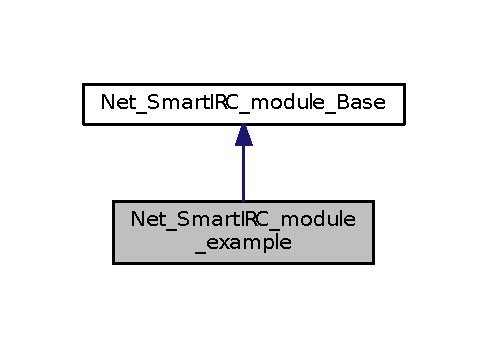
\includegraphics[width=205pt]{dd/de7/classNet__SmartIRC__module__example__inherit__graph}
\end{center}
\end{figure}


Collaboration diagram for Net\+\_\+\+Smart\+I\+R\+C\+\_\+module\+\_\+example\+:
\nopagebreak
\begin{figure}[H]
\begin{center}
\leavevmode
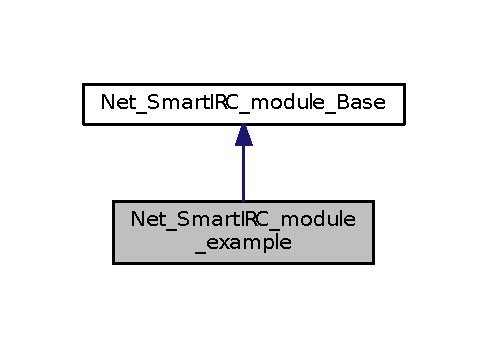
\includegraphics[width=205pt]{df/de1/classNet__SmartIRC__module__example__coll__graph}
\end{center}
\end{figure}
\subsection*{Public Member Functions}
\begin{DoxyCompactItemize}
\item 
\hyperlink{classNet__SmartIRC__module__example_a314c836af3c9d8950164bf7d9bb785d6}{\+\_\+\+\_\+construct} (\$irc)
\item 
\hyperlink{classNet__SmartIRC__module__example_a20445df064117b852223745ba9a2aa22}{\+\_\+\+\_\+destruct} ()
\end{DoxyCompactItemize}
\subsection*{Public Attributes}
\begin{DoxyCompactItemize}
\item 
\hyperlink{classNet__SmartIRC__module__example_aaebd09582fd081d9afff44777c85c8d8}{\$name} = \textquotesingle{}\textquotesingle{}
\item 
\hyperlink{classNet__SmartIRC__module__example_a84a5abd912985d58483093ee128d6aed}{\$author} = \textquotesingle{}\textquotesingle{}
\item 
\hyperlink{classNet__SmartIRC__module__example_ae66fb76a41befbcdb9ba370dd2a8aafd}{\$description} = \textquotesingle{}\textquotesingle{}
\item 
\hyperlink{classNet__SmartIRC__module__example_a768e94b6407b8020f8d388507ba3fbe1}{\$license} = \textquotesingle{}M\+IT\textquotesingle{}
\end{DoxyCompactItemize}
\subsection*{Private Attributes}
\begin{DoxyCompactItemize}
\item 
\hyperlink{classNet__SmartIRC__module__example_a2d7ea47e77c4dc79aff1c43200e54c82}{\$irc}
\end{DoxyCompactItemize}


\subsection{Detailed Description}
Create a bot module to be used by Net\+\_\+\+Smart\+I\+RC library. Change the name of the class after \char`\"{}\+Net\+\_\+\+Smart\+I\+R\+C\+\_\+module\+\_\+\char`\"{} to match the botname. e.\+g. If your botname is \char`\"{}robo\char`\"{}, class name should be Net\+\_\+\+Smart\+I\+R\+C\+\_\+module\+\_\+robo. Note names are case-\/sensitive. 

\subsection{Constructor \& Destructor Documentation}
\index{Net\+\_\+\+Smart\+I\+R\+C\+\_\+module\+\_\+example@{Net\+\_\+\+Smart\+I\+R\+C\+\_\+module\+\_\+example}!\+\_\+\+\_\+construct@{\+\_\+\+\_\+construct}}
\index{\+\_\+\+\_\+construct@{\+\_\+\+\_\+construct}!Net\+\_\+\+Smart\+I\+R\+C\+\_\+module\+\_\+example@{Net\+\_\+\+Smart\+I\+R\+C\+\_\+module\+\_\+example}}
\subsubsection[{\texorpdfstring{\+\_\+\+\_\+construct(\$irc)}{__construct($irc)}}]{\setlength{\rightskip}{0pt plus 5cm}Net\+\_\+\+Smart\+I\+R\+C\+\_\+module\+\_\+example\+::\+\_\+\+\_\+construct (
\begin{DoxyParamCaption}
\item[{}]{\$irc}
\end{DoxyParamCaption}
)}\hypertarget{classNet__SmartIRC__module__example_a314c836af3c9d8950164bf7d9bb785d6}{}\label{classNet__SmartIRC__module__example_a314c836af3c9d8950164bf7d9bb785d6}
Constructor. 
\begin{DoxyParams}{Parameters}
{\em \$irc} & (object). \\
\hline
\end{DoxyParams}
\index{Net\+\_\+\+Smart\+I\+R\+C\+\_\+module\+\_\+example@{Net\+\_\+\+Smart\+I\+R\+C\+\_\+module\+\_\+example}!\+\_\+\+\_\+destruct@{\+\_\+\+\_\+destruct}}
\index{\+\_\+\+\_\+destruct@{\+\_\+\+\_\+destruct}!Net\+\_\+\+Smart\+I\+R\+C\+\_\+module\+\_\+example@{Net\+\_\+\+Smart\+I\+R\+C\+\_\+module\+\_\+example}}
\subsubsection[{\texorpdfstring{\+\_\+\+\_\+destruct()}{__destruct()}}]{\setlength{\rightskip}{0pt plus 5cm}Net\+\_\+\+Smart\+I\+R\+C\+\_\+module\+\_\+example\+::\+\_\+\+\_\+destruct (
\begin{DoxyParamCaption}
{}
\end{DoxyParamCaption}
)}\hypertarget{classNet__SmartIRC__module__example_a20445df064117b852223745ba9a2aa22}{}\label{classNet__SmartIRC__module__example_a20445df064117b852223745ba9a2aa22}
Call parent destructor. 

\subsection{Member Data Documentation}
\index{Net\+\_\+\+Smart\+I\+R\+C\+\_\+module\+\_\+example@{Net\+\_\+\+Smart\+I\+R\+C\+\_\+module\+\_\+example}!\$author@{\$author}}
\index{\$author@{\$author}!Net\+\_\+\+Smart\+I\+R\+C\+\_\+module\+\_\+example@{Net\+\_\+\+Smart\+I\+R\+C\+\_\+module\+\_\+example}}
\subsubsection[{\texorpdfstring{\$author}{$author}}]{\setlength{\rightskip}{0pt plus 5cm}Net\+\_\+\+Smart\+I\+R\+C\+\_\+module\+\_\+example\+::\$author = \textquotesingle{}\textquotesingle{}}\hypertarget{classNet__SmartIRC__module__example_a84a5abd912985d58483093ee128d6aed}{}\label{classNet__SmartIRC__module__example_a84a5abd912985d58483093ee128d6aed}
\index{Net\+\_\+\+Smart\+I\+R\+C\+\_\+module\+\_\+example@{Net\+\_\+\+Smart\+I\+R\+C\+\_\+module\+\_\+example}!\$description@{\$description}}
\index{\$description@{\$description}!Net\+\_\+\+Smart\+I\+R\+C\+\_\+module\+\_\+example@{Net\+\_\+\+Smart\+I\+R\+C\+\_\+module\+\_\+example}}
\subsubsection[{\texorpdfstring{\$description}{$description}}]{\setlength{\rightskip}{0pt plus 5cm}Net\+\_\+\+Smart\+I\+R\+C\+\_\+module\+\_\+example\+::\$description = \textquotesingle{}\textquotesingle{}}\hypertarget{classNet__SmartIRC__module__example_ae66fb76a41befbcdb9ba370dd2a8aafd}{}\label{classNet__SmartIRC__module__example_ae66fb76a41befbcdb9ba370dd2a8aafd}
\index{Net\+\_\+\+Smart\+I\+R\+C\+\_\+module\+\_\+example@{Net\+\_\+\+Smart\+I\+R\+C\+\_\+module\+\_\+example}!\$irc@{\$irc}}
\index{\$irc@{\$irc}!Net\+\_\+\+Smart\+I\+R\+C\+\_\+module\+\_\+example@{Net\+\_\+\+Smart\+I\+R\+C\+\_\+module\+\_\+example}}
\subsubsection[{\texorpdfstring{\$irc}{$irc}}]{\setlength{\rightskip}{0pt plus 5cm}Net\+\_\+\+Smart\+I\+R\+C\+\_\+module\+\_\+example\+::\$irc\hspace{0.3cm}{\ttfamily [private]}}\hypertarget{classNet__SmartIRC__module__example_a2d7ea47e77c4dc79aff1c43200e54c82}{}\label{classNet__SmartIRC__module__example_a2d7ea47e77c4dc79aff1c43200e54c82}
\index{Net\+\_\+\+Smart\+I\+R\+C\+\_\+module\+\_\+example@{Net\+\_\+\+Smart\+I\+R\+C\+\_\+module\+\_\+example}!\$license@{\$license}}
\index{\$license@{\$license}!Net\+\_\+\+Smart\+I\+R\+C\+\_\+module\+\_\+example@{Net\+\_\+\+Smart\+I\+R\+C\+\_\+module\+\_\+example}}
\subsubsection[{\texorpdfstring{\$license}{$license}}]{\setlength{\rightskip}{0pt plus 5cm}Net\+\_\+\+Smart\+I\+R\+C\+\_\+module\+\_\+example\+::\$license = \textquotesingle{}M\+IT\textquotesingle{}}\hypertarget{classNet__SmartIRC__module__example_a768e94b6407b8020f8d388507ba3fbe1}{}\label{classNet__SmartIRC__module__example_a768e94b6407b8020f8d388507ba3fbe1}
\index{Net\+\_\+\+Smart\+I\+R\+C\+\_\+module\+\_\+example@{Net\+\_\+\+Smart\+I\+R\+C\+\_\+module\+\_\+example}!\$name@{\$name}}
\index{\$name@{\$name}!Net\+\_\+\+Smart\+I\+R\+C\+\_\+module\+\_\+example@{Net\+\_\+\+Smart\+I\+R\+C\+\_\+module\+\_\+example}}
\subsubsection[{\texorpdfstring{\$name}{$name}}]{\setlength{\rightskip}{0pt plus 5cm}Net\+\_\+\+Smart\+I\+R\+C\+\_\+module\+\_\+example\+::\$name = \textquotesingle{}\textquotesingle{}}\hypertarget{classNet__SmartIRC__module__example_aaebd09582fd081d9afff44777c85c8d8}{}\label{classNet__SmartIRC__module__example_aaebd09582fd081d9afff44777c85c8d8}


The documentation for this class was generated from the following file\+:\begin{DoxyCompactItemize}
\item 
bots/example/\hyperlink{example_2module_8php}{module.\+php}\end{DoxyCompactItemize}

\hypertarget{classNet__SmartIRC__module__shabri}{}\section{Net\+\_\+\+Smart\+I\+R\+C\+\_\+module\+\_\+shabri Class Reference}
\label{classNet__SmartIRC__module__shabri}\index{Net\+\_\+\+Smart\+I\+R\+C\+\_\+module\+\_\+shabri@{Net\+\_\+\+Smart\+I\+R\+C\+\_\+module\+\_\+shabri}}


Inheritance diagram for Net\+\_\+\+Smart\+I\+R\+C\+\_\+module\+\_\+shabri\+:
\nopagebreak
\begin{figure}[H]
\begin{center}
\leavevmode
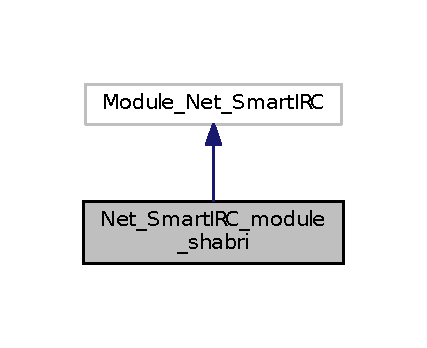
\includegraphics[width=205pt]{d5/d63/classNet__SmartIRC__module__shabri__inherit__graph}
\end{center}
\end{figure}


Collaboration diagram for Net\+\_\+\+Smart\+I\+R\+C\+\_\+module\+\_\+shabri\+:
\nopagebreak
\begin{figure}[H]
\begin{center}
\leavevmode
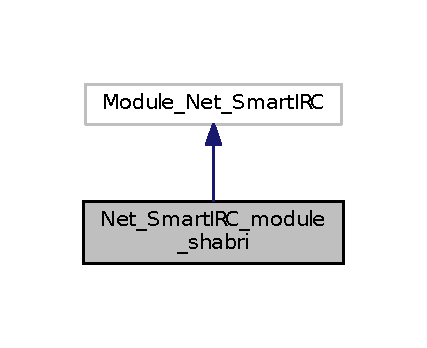
\includegraphics[width=205pt]{d4/d39/classNet__SmartIRC__module__shabri__coll__graph}
\end{center}
\end{figure}
\subsection*{Public Member Functions}
\begin{DoxyCompactItemize}
\item 
\hyperlink{classNet__SmartIRC__module__shabri_ac40c957f3dca3221a8e8efdc8bf29049}{\+\_\+\+\_\+construct} (\$irc)
\item 
\hyperlink{classNet__SmartIRC__module__shabri_ad51f5f82743d89efbe3c611d65757f0b}{\+\_\+\+\_\+destruct} ()
\end{DoxyCompactItemize}
\subsection*{Public Attributes}
\begin{DoxyCompactItemize}
\item 
\hyperlink{classNet__SmartIRC__module__shabri_a03db7b1894653334db45217284781a32}{\$name} = \textquotesingle{}\textquotesingle{}
\item 
\hyperlink{classNet__SmartIRC__module__shabri_a1fde51b8caf0d0cd8631c47ee16ae501}{\$author} = \textquotesingle{}\textquotesingle{}
\item 
\hyperlink{classNet__SmartIRC__module__shabri_af61d6f8235505952dbe0922ce1524412}{\$description} = \textquotesingle{}\textquotesingle{}
\item 
\hyperlink{classNet__SmartIRC__module__shabri_a08fcbcccb2c24469862e98cba1911049}{\$license} = \textquotesingle{}M\+IT\textquotesingle{}
\end{DoxyCompactItemize}
\subsection*{Private Attributes}
\begin{DoxyCompactItemize}
\item 
\hyperlink{classNet__SmartIRC__module__shabri_a6f5d61be96fc20ee5ffc8d07ccb2d578}{\$irc}
\end{DoxyCompactItemize}


\subsection{Detailed Description}
Create a bot module to be used by Net\+\_\+\+Smart\+I\+RC library. 

\subsection{Constructor \& Destructor Documentation}
\index{Net\+\_\+\+Smart\+I\+R\+C\+\_\+module\+\_\+shabri@{Net\+\_\+\+Smart\+I\+R\+C\+\_\+module\+\_\+shabri}!\+\_\+\+\_\+construct@{\+\_\+\+\_\+construct}}
\index{\+\_\+\+\_\+construct@{\+\_\+\+\_\+construct}!Net\+\_\+\+Smart\+I\+R\+C\+\_\+module\+\_\+shabri@{Net\+\_\+\+Smart\+I\+R\+C\+\_\+module\+\_\+shabri}}
\subsubsection[{\texorpdfstring{\+\_\+\+\_\+construct(\$irc)}{__construct($irc)}}]{\setlength{\rightskip}{0pt plus 5cm}Net\+\_\+\+Smart\+I\+R\+C\+\_\+module\+\_\+shabri\+::\+\_\+\+\_\+construct (
\begin{DoxyParamCaption}
\item[{}]{\$irc}
\end{DoxyParamCaption}
)}\hypertarget{classNet__SmartIRC__module__shabri_ac40c957f3dca3221a8e8efdc8bf29049}{}\label{classNet__SmartIRC__module__shabri_ac40c957f3dca3221a8e8efdc8bf29049}
Constructor. 
\begin{DoxyParams}{Parameters}
{\em \$irc} & (object). \\
\hline
\end{DoxyParams}
\index{Net\+\_\+\+Smart\+I\+R\+C\+\_\+module\+\_\+shabri@{Net\+\_\+\+Smart\+I\+R\+C\+\_\+module\+\_\+shabri}!\+\_\+\+\_\+destruct@{\+\_\+\+\_\+destruct}}
\index{\+\_\+\+\_\+destruct@{\+\_\+\+\_\+destruct}!Net\+\_\+\+Smart\+I\+R\+C\+\_\+module\+\_\+shabri@{Net\+\_\+\+Smart\+I\+R\+C\+\_\+module\+\_\+shabri}}
\subsubsection[{\texorpdfstring{\+\_\+\+\_\+destruct()}{__destruct()}}]{\setlength{\rightskip}{0pt plus 5cm}Net\+\_\+\+Smart\+I\+R\+C\+\_\+module\+\_\+shabri\+::\+\_\+\+\_\+destruct (
\begin{DoxyParamCaption}
{}
\end{DoxyParamCaption}
)}\hypertarget{classNet__SmartIRC__module__shabri_ad51f5f82743d89efbe3c611d65757f0b}{}\label{classNet__SmartIRC__module__shabri_ad51f5f82743d89efbe3c611d65757f0b}
Call parent destructor. 

\subsection{Member Data Documentation}
\index{Net\+\_\+\+Smart\+I\+R\+C\+\_\+module\+\_\+shabri@{Net\+\_\+\+Smart\+I\+R\+C\+\_\+module\+\_\+shabri}!\$author@{\$author}}
\index{\$author@{\$author}!Net\+\_\+\+Smart\+I\+R\+C\+\_\+module\+\_\+shabri@{Net\+\_\+\+Smart\+I\+R\+C\+\_\+module\+\_\+shabri}}
\subsubsection[{\texorpdfstring{\$author}{$author}}]{\setlength{\rightskip}{0pt plus 5cm}Net\+\_\+\+Smart\+I\+R\+C\+\_\+module\+\_\+shabri\+::\$author = \textquotesingle{}\textquotesingle{}}\hypertarget{classNet__SmartIRC__module__shabri_a1fde51b8caf0d0cd8631c47ee16ae501}{}\label{classNet__SmartIRC__module__shabri_a1fde51b8caf0d0cd8631c47ee16ae501}
\index{Net\+\_\+\+Smart\+I\+R\+C\+\_\+module\+\_\+shabri@{Net\+\_\+\+Smart\+I\+R\+C\+\_\+module\+\_\+shabri}!\$description@{\$description}}
\index{\$description@{\$description}!Net\+\_\+\+Smart\+I\+R\+C\+\_\+module\+\_\+shabri@{Net\+\_\+\+Smart\+I\+R\+C\+\_\+module\+\_\+shabri}}
\subsubsection[{\texorpdfstring{\$description}{$description}}]{\setlength{\rightskip}{0pt plus 5cm}Net\+\_\+\+Smart\+I\+R\+C\+\_\+module\+\_\+shabri\+::\$description = \textquotesingle{}\textquotesingle{}}\hypertarget{classNet__SmartIRC__module__shabri_af61d6f8235505952dbe0922ce1524412}{}\label{classNet__SmartIRC__module__shabri_af61d6f8235505952dbe0922ce1524412}
\index{Net\+\_\+\+Smart\+I\+R\+C\+\_\+module\+\_\+shabri@{Net\+\_\+\+Smart\+I\+R\+C\+\_\+module\+\_\+shabri}!\$irc@{\$irc}}
\index{\$irc@{\$irc}!Net\+\_\+\+Smart\+I\+R\+C\+\_\+module\+\_\+shabri@{Net\+\_\+\+Smart\+I\+R\+C\+\_\+module\+\_\+shabri}}
\subsubsection[{\texorpdfstring{\$irc}{$irc}}]{\setlength{\rightskip}{0pt plus 5cm}Net\+\_\+\+Smart\+I\+R\+C\+\_\+module\+\_\+shabri\+::\$irc\hspace{0.3cm}{\ttfamily [private]}}\hypertarget{classNet__SmartIRC__module__shabri_a6f5d61be96fc20ee5ffc8d07ccb2d578}{}\label{classNet__SmartIRC__module__shabri_a6f5d61be96fc20ee5ffc8d07ccb2d578}
\index{Net\+\_\+\+Smart\+I\+R\+C\+\_\+module\+\_\+shabri@{Net\+\_\+\+Smart\+I\+R\+C\+\_\+module\+\_\+shabri}!\$license@{\$license}}
\index{\$license@{\$license}!Net\+\_\+\+Smart\+I\+R\+C\+\_\+module\+\_\+shabri@{Net\+\_\+\+Smart\+I\+R\+C\+\_\+module\+\_\+shabri}}
\subsubsection[{\texorpdfstring{\$license}{$license}}]{\setlength{\rightskip}{0pt plus 5cm}Net\+\_\+\+Smart\+I\+R\+C\+\_\+module\+\_\+shabri\+::\$license = \textquotesingle{}M\+IT\textquotesingle{}}\hypertarget{classNet__SmartIRC__module__shabri_a08fcbcccb2c24469862e98cba1911049}{}\label{classNet__SmartIRC__module__shabri_a08fcbcccb2c24469862e98cba1911049}
\index{Net\+\_\+\+Smart\+I\+R\+C\+\_\+module\+\_\+shabri@{Net\+\_\+\+Smart\+I\+R\+C\+\_\+module\+\_\+shabri}!\$name@{\$name}}
\index{\$name@{\$name}!Net\+\_\+\+Smart\+I\+R\+C\+\_\+module\+\_\+shabri@{Net\+\_\+\+Smart\+I\+R\+C\+\_\+module\+\_\+shabri}}
\subsubsection[{\texorpdfstring{\$name}{$name}}]{\setlength{\rightskip}{0pt plus 5cm}Net\+\_\+\+Smart\+I\+R\+C\+\_\+module\+\_\+shabri\+::\$name = \textquotesingle{}\textquotesingle{}}\hypertarget{classNet__SmartIRC__module__shabri_a03db7b1894653334db45217284781a32}{}\label{classNet__SmartIRC__module__shabri_a03db7b1894653334db45217284781a32}


The documentation for this class was generated from the following file\+:\begin{DoxyCompactItemize}
\item 
bots/shabri/\hyperlink{shabri_2module_8php}{module.\+php}\end{DoxyCompactItemize}

\chapter{File Documentation}
\hypertarget{example_2module_8php}{}\section{bots/example/module.php File Reference}
\label{example_2module_8php}\index{bots/example/module.\+php@{bots/example/module.\+php}}
\subsection*{Classes}
\begin{DoxyCompactItemize}
\item 
class \hyperlink{classNet__SmartIRC__module__example}{Net\+\_\+\+Smart\+I\+R\+C\+\_\+module\+\_\+example}
\end{DoxyCompactItemize}


\subsection{Detailed Description}
Bot module. Extend of modify this class to add more functionality to your bot. 
\hypertarget{shabri_2module_8php}{}\section{bots/shabri/module.php File Reference}
\label{shabri_2module_8php}\index{bots/shabri/module.\+php@{bots/shabri/module.\+php}}
\subsection*{Classes}
\begin{DoxyCompactItemize}
\item 
class \hyperlink{classNet__SmartIRC__module__shabri}{Net\+\_\+\+Smart\+I\+R\+C\+\_\+module\+\_\+shabri}
\end{DoxyCompactItemize}


\subsection{Detailed Description}
Bot module. Extend of modify this class to add more functionality to your bot. 
%--- End generated contents ---

% Index
\backmatter
\newpage
\phantomsection
\clearemptydoublepage
\addcontentsline{toc}{chapter}{Index}
\printindex

\end{document}
